\clearpage



\begin{appendix}
\section{}
\hypertarget{appendix-e}{%
\subsection{}\label{appendix-e}}

\begin{figure*}

{\centering 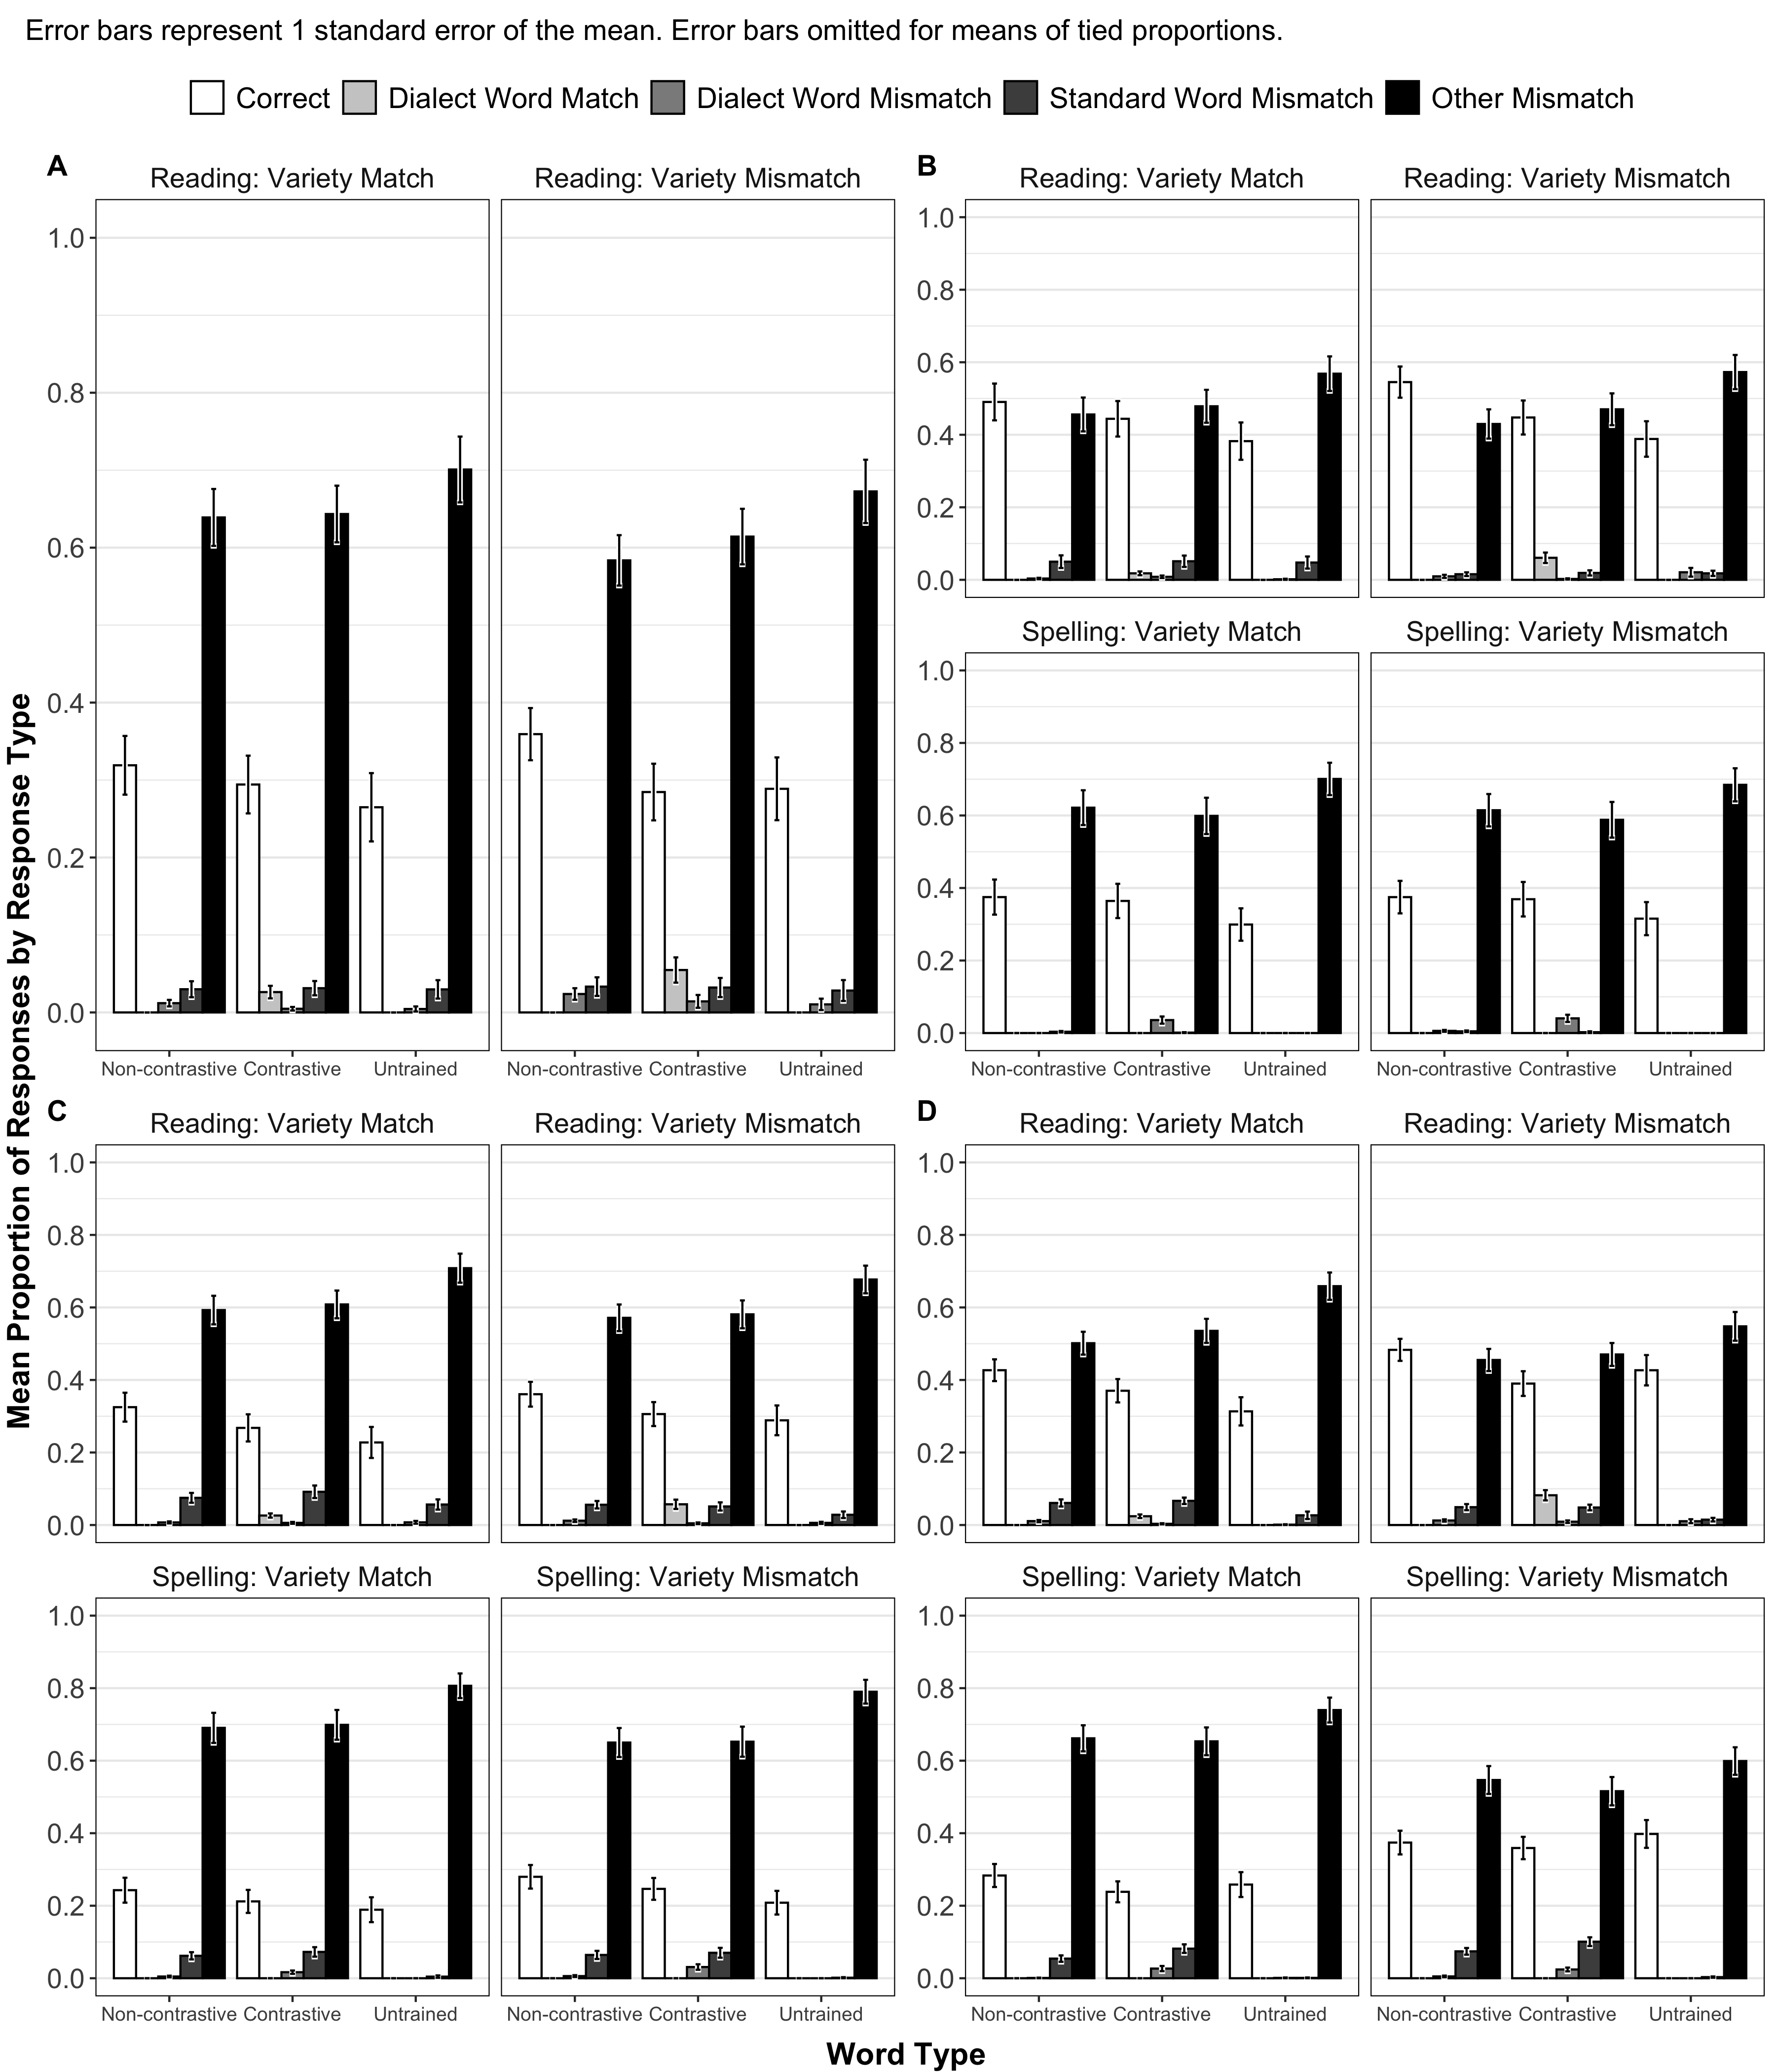
\includegraphics[width=0.8\linewidth]{/Users/glennwilliams/Dropbox/GitHub/levenik/03_analysis/05_exploratory-analysis/output/plots/combined_mean_proportions} 

}

\caption{Mean proportion of response types for Experiments 1 (panel A), 2a (panel B), 2b (panel C), and 3 (panel D). Response types are: correct (e.g. target: \textit{kuble}--response: \textit{kuble}); dialect word match: the dialect variant is produced in response to the corresponding standard contrastive word (e.g. target: \textit{kuble}--response: \textit{xuble}); dialect word misatch: a dialect variant is produced in response to another standard contrastive word (e.g. target: \textit{skefi}--response: \textit{xuble}); standard word mismatch: a standard word is produced in response to another standard word (e.g. target: \textit{skefi}--response: \textit{kuble}); other mismatch: any other error that was not part of the response set.}(\#fig:unnamed-chunk-7)
\end{figure*}
\end{appendix}
